\section{Experimentation and results}\label{experimentations}
We detail and analyze in the section the results of the experimentation we performed using the six ML algorithms presented in Section \ref{ml_algorithms} over the two real datasets described in Section \ref{datasets}. We start by presenting our experimentation setting.

% experimentation setting
\subsection{Experimentation Setting}
In this section data is available for applying classification algorithm. After model creation from training data, classification operation is performed on test data. 
All the performed tests have been done in the same machine and the same operating system. To test the performance of our six chosen ML algorithms, we relied on their Python implementations available through the scikit-learn library. Scikit-learn is an open source simple and efficient tool for predictive data analysis that implements most of the existing ML algorithms

Then some of the most important performance evaluation measures like accuracy, precision, sensitivity, specificity, F-measure and area under ROC curve are evaluated and compared. 
For the details about the description of each parameter of ML we refer to the official documentation of the implementation of these algorithms in scikit-learn7. Concerning the segmentation of both datasets for the training of our ML algorithms and their testing we have considered the stratified-5-fold cross-validation in classification model construction and efficiency evaluation. This method is very useful to handle data with an unbalanced class distribution, increases the validation of classification and prevents from random and invalid results.


% Results of the experiments
\subsection{Results of the experiments}

This section presents the results of the experimentation on each real dataset for each of the six classifiers. 
\subsubsection{Decision Tree}

Table 1  below shows the performance measures (precision, recall, F measure and precision) of the results of our Decision Tree classifier after experimentation on all our datasets. The observation shows that the best scores of our classifier are achieved on the datasets DT1, DT3 and DT5 which are 97.04\%, 80.86\% and 83.41\% respectively. Also AUC (Area Under the Curve) values are higher for these same datasets which are 0.78, 0.86 and 0.76 respectively. However, we note that the sensitivity values are higher than the specificity values on the datasets DT1, DT3  and DT5 whereas they are substantially lower than thoses of datasets DT2 and DT4. This means that DT is more inclined to predict as well whether a given patient has malaria or he doesn’t, on the datasets DT2, DT3 and DT4, while our classifier on the datasets DT1 and DT5 our classifier is only efficient in predicting whether a given patient has malaria. This same trend is observed on the F-scores which higher values varying between 0.91 and 0.98 on the datasets DT1, DT3 and DT5.

% Decision Tree
\begin{table}[!ht]
\centering
\begin{tabular}{*{7}{c}l r}
  \toprule
  \textbf{Datasets} & \textbf{Precision} & \textbf{Recall} & \textbf{F1-score}&\textbf{AUC} &\textbf{Score}&\textbf{Specificity}\\
   \midrule
  DT1 &0.97  & 1   & 0.98 & 0.78 & 97.04 & 0.05 \\
  DT2 & 0.59 &0.48 &0.48  &0.64  &63.01  &0.80\\
  DT3 &0.89  &0.85 &0.87  &0.86  &80.86  &0.69\\
  DT4 &0.68  &0.57 &0.62  &0.70  &65.60  &0.74\\
  DT5 &0.99  &0.84 &0.91  &0.76  &83.41  &0.58\\

  
    \bottomrule
\end{tabular}
\caption{Performances measures of DT over all datasets}\label{perf-measure-dt1}
\end{table}
\subsubsection{Random Forest}
The performance of the random forest varied throughout the study depending on the dataset, although overall it performed well as shown in Table 2. Notice that best accuracy are achieved by random forest classifier on the datasets DT1, DT2 and DT5 which are respectively 97.13\%, 80.86\% and 78.35\%. In contrast with the results obtained with the DT classifier, the Sensivity values are higher than specificity values on datasets DT1 and DT5 whereas the inverse is noticed on the dataset DT3. At the same time we note that these values are roughly identical on the datasets DT3 and D4
%Random Forest
\begin{table}[!ht]
\centering
\begin{tabular}{*{7}{c}l r}
  \toprule
  \textbf{Datasets} & \textbf{Precision} & \textbf{Recall} & \textbf{F1-score}&\textbf{AUC} &\textbf{Score} &\textbf{Specificity}\\
   \midrule
  DT1 &0.97 &1   &0.99 &0.81 &97.13& 0.07\\
  DT2 &0.63  & 0.34  &0.44&0.64&63.33& 0.85\\
  DT3 &0.89 &0.85 &0.87&087&80.86&0.70\\
  DT4 &0.68 &0.56&0.62&0.70&65.82&0.74\\
  DT5 &0.99 &0.84&0.91&0.76&78.35&0.60\\
  
  
    \bottomrule
\end{tabular}
\caption{Performances measures of RF over all datasets}\label{perf-measure-dt1}
\end{table}


%Logistic Regression
\subsubsection{Logistic Regression}

Logistic regression In table 3 we show the performance measures LR classifier experimented on our five datasets. We notice that our classifier have overall precision which are vary between 58\% and 98\%. 

\begin{table}[!ht]
\centering
\begin{tabular}{*{7}{c}l r}
  \toprule
  \textbf{Datasets} & \textbf{Precision} & \textbf{Recall} & \textbf{F1-score}&\textbf{AUC} &\textbf{Score}&\textbf{Specificity}\\
   \midrule
  DT1 &0.97 &1   &0.99 &0.79 &97.19&0.05 \\
  DT2 & 0.58 &0.36   &0.44&0.63&61.96&0.81\\
  DT3 &0.85 &0.88 &0.86&0.86&79.59&0.55\\
  DT4 &0.98 &0.56&0.92&0.70&65.82&0.72\\
  DT5 & 0.90&0.78&0.88&0.84&81.86&0.75\\
  
  
    \bottomrule
\end{tabular}
\caption{Performances measures of LR over all datasets}\label{perf-measure-dt1}
\end{table}
We observe that the higher precision is obtained with DT4 dataset while the corresponding score is equal to 65.82\% is the lowest of all other datasets. Also we notice that the LR presents homogeneous results on the DT3 dataset with an accuracy of 85\%, a sensitivity equal to 88\%, an F-score of 92\%, an AUC which is 0.86 and a score equal to 79.59\%. . We also note that the best AUC and the best F-score are obtained by LR on the DT3 dataset.
\subsubsection{Naives Bayes}
In contrast with the results above, NB classifier presents very heterogeneous performances regarding the performance measures used as shown in Table 4. In fact, we observe that the best precision is achieved on the dataset DT5 which is 99\%, although the best F-score and the higher accuracy are obtained on the dataset DT1 which are 0.99 and 97.13\% respectively and finally the best AUC is observed on the dataset DT3 which is 0.85. We also note that the best specificity is obtained on DT4 and varies between 0.65 and 0.70 (see appendices).
\begin{table}[!ht]
\centering
\begin{tabular}{*{7}{c}l r}
  \toprule
  \textbf{Datasets} & \textbf{Precision} & \textbf{Recall} & \textbf{F1-score}&\textbf{AUC} &\textbf{Score}&\textbf{Specificity}\\
   \midrule
  DT1 &0.97 &1   &0.99 &0.81 &97.13 &0.00\\
  DT2 & 0.60 &0.34   &0.43&0.63&62.86&0.83 \\
  DT3 &0.86 &0.87 &0.86&0.85&79.94&0.60\\
  DT4 &0.68 &0.59&0.63&0.70&65.63&0.73\\
  DT5 &0.99 &0.82&0.90&0.84&85.61&0.71\\
  
  
    \bottomrule
\end{tabular}
\caption{Performances measures of NB over all datasets}\label{perf-measure-dt1}
\end{table}
\subsubsection{Support Vector Machine}
%SVM

Table 5 shows the performance measures of the SVM classifier.
\begin{table}[!ht]
\centering
\begin{tabular}{*{7}{c}l r}
  \toprule
  \textbf{Datasets} & \textbf{Precision} & \textbf{Recall} & \textbf{F1-score}&\textbf{AUC} &\textbf{Score}&\textbf{Specificity}\\
   \midrule
  DT1 &0.97 &1   &0.99 &0.84 &97.13&0.00 \\
  DT2 &0.58  &0.05   & 0.09&0.62&62.86&0.97\\
  DT3 &0.57 & 0.86&0.86&0.85&79.94&0.64\\
  DT4 & 0.68&0.58&0.62&0.70&65.63&0.73\\
  DT5 &0.99 &0.86&0.92&0.80&85.61&0.62\\
    \bottomrule
\end{tabular}
\caption{Performances measures of SVM over all datasets}\label{perf-measure-dt1}
\end{table}
Table 1 shows the performance measures. The observation shows that the best score, precision and F1-score are obtained on the datasets DT1, DT3 and DT5. However the higher AUC and the best specificity are observer on the datasets DT1, DT3 and DT4.
%ANN
\subsubsection{Artificial Neural Nework}
The performance of the ANN varied throughout the study depending on the dataset, although overall it performed well. A large amount of initial effort was required to train and validate the model. Notice that best precision are achieved by ANN classifier on the datasets DT1, DT3 and DT5 which are respectively 97\%, 89\% and 99\%. While the higher AUC and the best scores are obtained on the datasets DT1 and DT3. The Sensivity values are higher than specificity values on datasets 
\begin{table}[!ht]
\centering
\begin{tabular}{*{8}{c}l r}
  \toprule
  \textbf{Datasets} & \textbf{Precision} & \textbf{Recall} & \textbf{F1-score}&\textbf{AUC} &\textbf{Score}&\textbf{Specificity}\\
   \midrule
  DT1 &0.97&1 &0.99   &0.84 &97.15&0.04  \\
  DT2 &0.59  &0.40   &0.48&0.65&62.86&0.80 \\
  DT3 &0.89 &0.85 &0.87&0.87&86.68&0.69\\
  DT4 &0.68 &0.58&0.62&0.70&0.70&0.75\\
  DT5 &0.99 &0.84&0.91&0.79&83.26&0.65\\ 
    \bottomrule
\end{tabular}
\caption{Performances measures of ANN over all datasets}\label{perf-measure-dt1}
\end{table}

\subsection{Discussion}
In this study, the algorithms DT, RF, LR, NB, SVM and ANN were applied on five datasets concerning patients with or without malaria and living in regions of Senegal namely: Diourbel, Thies and Fatick. Indeed, in order to offer a new technique for diagnosing and predicting malaria, it is important to know the performance of those existing through our datasets.
Analysing in details the performance of our six classifiers across the five datasets, the results show that there is not necessarily a single best classification algorithm, but that the best performing algorithm will depend on the characteristics of the dataset to analyze. Indeed we notice that all the algorithms produce their best precision on the DT1, DT3, and DT5 data sets. These values, which reach 97\% at times, outperform the Rapid Diagnosis Test which is the standard diagnostic tool largely adopted in the healthcare system in Senegal.
\begin{figure}
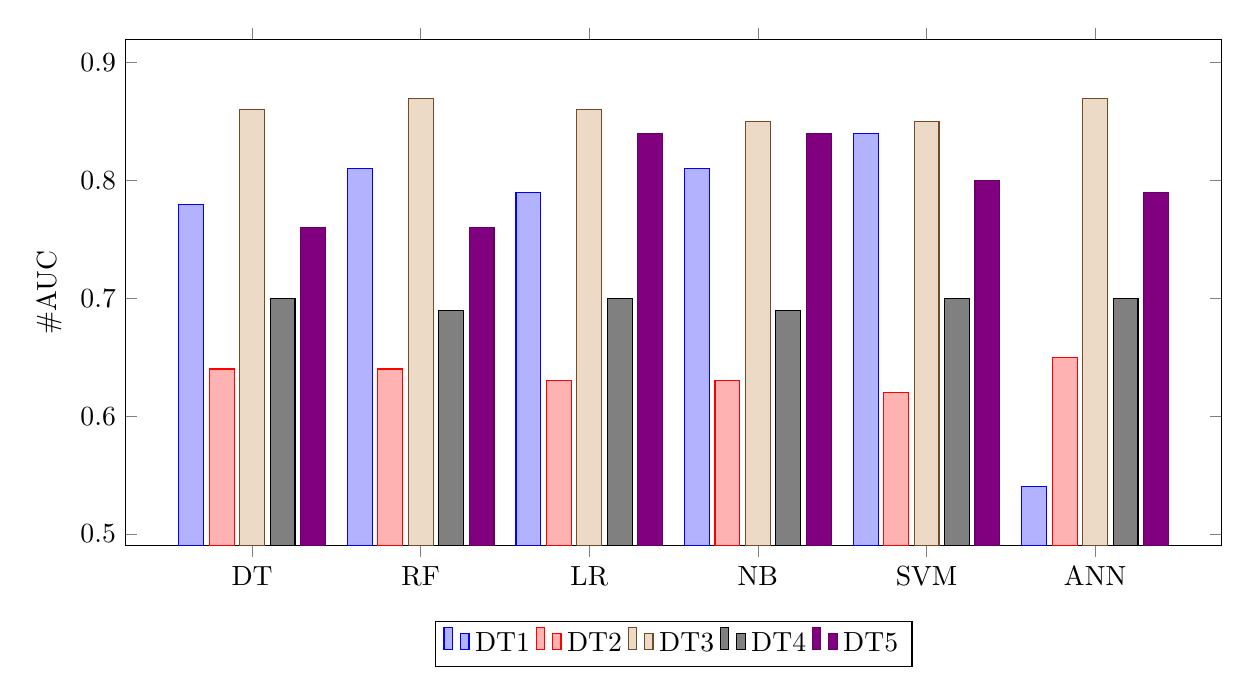
\begin{tikzpicture}
 \centering
\begin{axis}[
    height=8cm, width=15.5cm,
    bar width=0.4cm,
    ybar,
    %ybar=5pt,% configures `bar shift'
    bar width=9pt,
    enlargelimits=0.15,
    legend style={at={(0.5,-0.15)},
    anchor=north,legend columns=-1},
    ylabel={\#AUC},
    symbolic x coords={{DT,RF,LR,NB,SVM,ANN}},
    xtick=data,
    %nodes near coords,
    nodes near coords align={vertical},
    ]
\addplot coordinates {(DT,0.78) (RF, 0.81) (LR,0.79)(NB, 0.81)(SVM,0.84)(ANN, 0.54)};
\addplot coordinates{(DT,0.64) (RF, 0.64) (LR,0.63)(NB, 0.63)(SVM,0.62)(ANN, 0.65)};
\addplot coordinates {(DT,0.86) (RF, 0.87) (LR,0.86)(NB, 0.85)(SVM,0.85)(ANN, 0.87)};
\addplot coordinates {(DT,0.70) (RF, 0.69) (LR,0.70)(NB, 0.69)(SVM,0.70)(ANN, 0.70)};
\addplot coordinates {(DT,0.76) (RF, 0.76) (LR,0.84)(NB, 0.84)(SVM,0.80)(ANN, 0.79)};
\legend{DT1,DT2,DT3,DT4,DT5}
\end{axis}
\end{tikzpicture}
\caption{comparison of Roc Area achieved by six classifiers}
\end{figure}
However, on these same datasets, the algorithms often present very low specificities, for example 0.05 on DT1. This shows that our best performing classifiers are only able to predict a single class: either the patient has malaria or he does not, but not in both spots. This is because the DT1 and DT3 datasets are very unbalanced. In fact in these datasets either the number of patients with malaria is greater than those who are not or the opposite is true. Furthermore, we note that on the DT2 and DT4 datasets all the algorithms present specificities and Sensivity that are significant and quite similar. Contrary to what is quoted a little above, on these datasets the algorithms are efficient on the prediction tasks of the two classes. Looking closely at the results in terms of precision, recall and F-measure we observe that the classifiers RF, LR, SVM and ANN generally outperform the others for each dataset. Indeed, for the dataset DT1, which contains observations on patients living in different regions of Senegal, these four classifiers have an accuracy of 99\%, a recall greater than 92\% and an F-measure greater than 95\%. We note the same trend with the DT2 dataset which contains observations on patients living in the same area in Senegal. It can also be noted that RF, LR, SVM and ANN have better precision than the rapid diagnostic test carried out and systematically used in the majority of health structures in Senegal. This observation remains true with DT4 which is a perfectly balanced dataset. In conclusion, it is very difficult or even impossible for us to say definitively which algorithm is more efficient for the task of predicting malaria, but the choice of this one will strongly depend on the choice of the data set. However, this study shows that our classification problem has been taken care of. A method integrating several models and various datasets is necessary

\begin{figure}
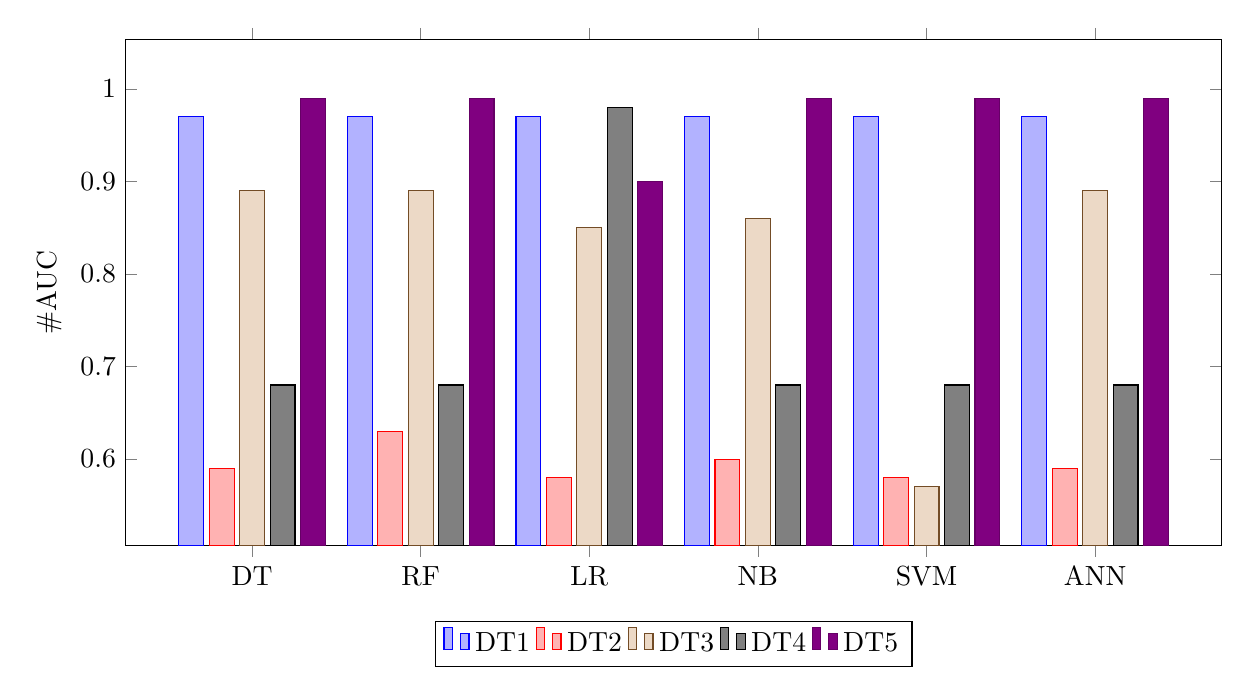
\begin{tikzpicture}
 \centering
\begin{axis}[
    height=8cm, width=15.5cm,
    bar width=0.4cm,
    ybar,
    %ybar=5pt,% configures `bar shift'
    bar width=9pt,
    enlargelimits=0.15,
    legend style={at={(0.5,-0.15)},
    anchor=north,legend columns=-1},
    ylabel={\#AUC},
    symbolic x coords={{DT,RF,LR,NB,SVM,ANN}},
    xtick=data,
    %nodes near coords,
    nodes near coords align={vertical},
    ]
\addplot coordinates {(DT,0.97) (RF, 0.97) (LR,0.97)(NB, 0.97)(SVM,0.97)(ANN, 0.97)};
\addplot coordinates{(DT,0.59) (RF, 0.63) (LR,0.58)(NB, 0.60)(SVM,0.58)(ANN, 0.59)};
\addplot coordinates {(DT,0.89) (RF, 0.89) (LR,0.85)(NB, 0.86)(SVM,0.57)(ANN, 0.89)};
\addplot coordinates {(DT,0.68) (RF, 0.68) (LR,0.98)(NB, 0.68)(SVM,0.68)(ANN, 0.68)};
\addplot coordinates {(DT,0.99) (RF, 0.99) (LR,0.90)(NB, 0.99)(SVM,0.99)(ANN, 0.99)};
\legend{DT1,DT2,DT3,DT4,DT5}
\end{axis}
\end{tikzpicture}
\caption{comparison of Precision achieved by six classifiers}

\end{figure}


\begin{figure}
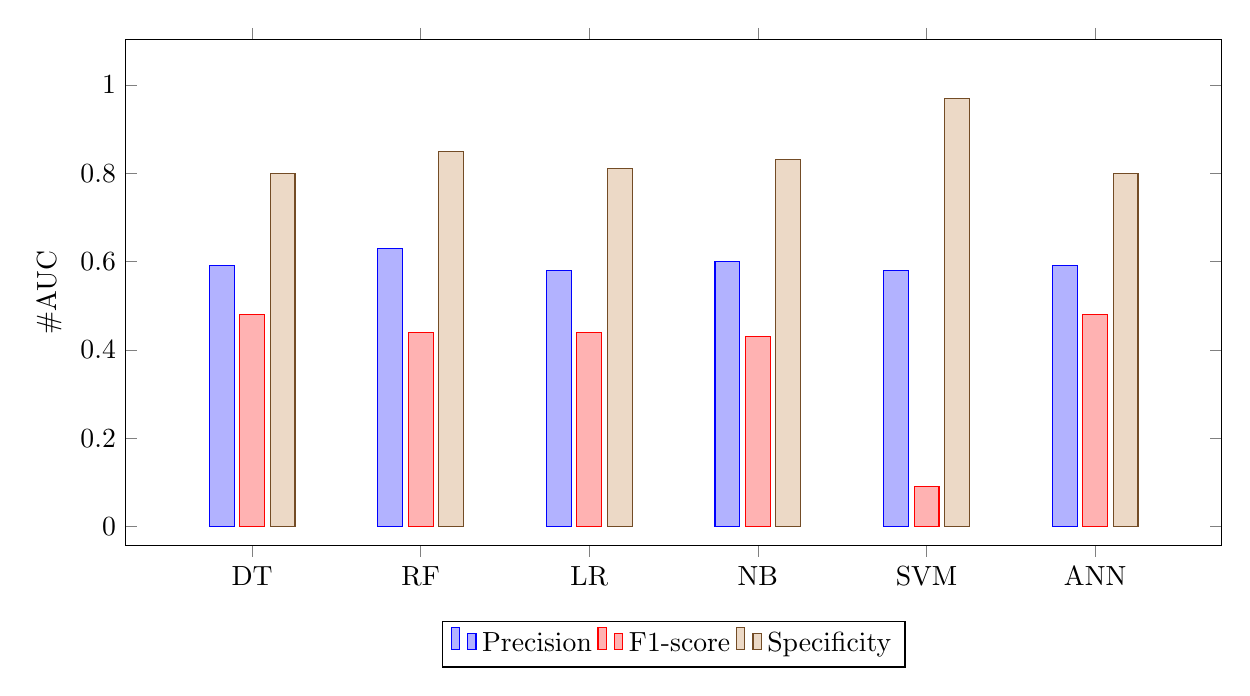
\begin{tikzpicture}
 \centering
\begin{axis}[
    height=8cm, width=15.5cm,
    bar width=0.4cm,
    ybar,
    %ybar=5pt,% configures `bar shift'
    bar width=9pt,
    enlargelimits=0.15,
    legend style={at={(0.5,-0.15)},
    anchor=north,legend columns=-1},
    ylabel={\#AUC},
    symbolic x coords={{DT,RF,LR,NB,SVM,ANN}},
    xtick=data,
    %nodes near coords,
    nodes near coords align={vertical},
    ]
\addplot coordinates {(DT,0.59) (RF, 0.63) (LR,0.58)(NB, 0.60)(SVM,0.58)(ANN, 0.59)};
\addplot coordinates{(DT,0.48) (RF, 0.44) (LR,0.44)(NB, 0.43)(SVM,0.09)(ANN, 0.48)};
\addplot coordinates {(DT,0.80) (RF, 0.85) (LR,0.81)(NB, 0.83)(SVM,0.97)(ANN, 0.80)};
%\addplot coordinates {(DT,0.68) (RF, 0.68) (LR,0.98)(NB, 0.68)(SVM,0.68)(ANN, 0.68)};
%\addplot coordinates {(DT,0.99) (RF, 0.99) (LR,0.90)(NB, 0.99)(SVM,0.99)(ANN, 0.99)};
\legend{Precision,F1-score,Specificity,DT4}
\end{axis}
\end{tikzpicture}
\caption{comparison of other performance measures in classifiers on DT1}

\end{figure}